\textbf{3-1.}如习题 3-1 图所示,一小车沿倾角为 $\theta$ 的光滑斜面滑下。小车上悬挂一摆锤。当摆锤相对小车静止时,摆线与竖直线的夹角为多大?

\begin{figure}[H]
  \centering
  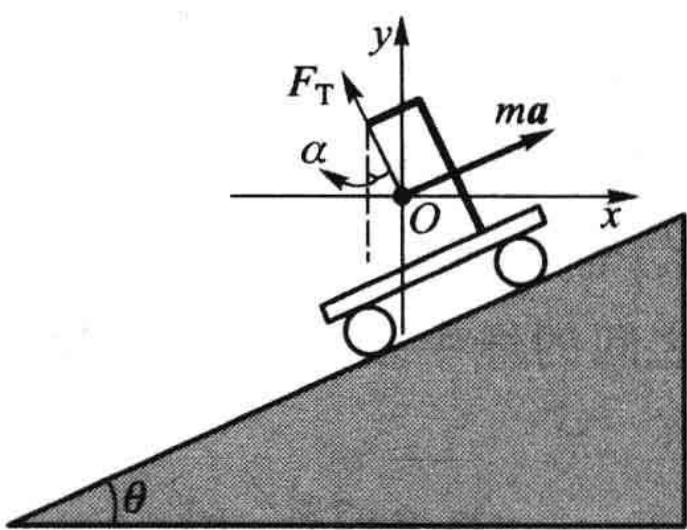
\includegraphics[width=0.25\textwidth]{figures/fig3-1_x.jpg}
  \end{figure}

\vfill

\textbf{3-2.}在卡车的尾部通过一根绳子拖着一根粗细均匀的圆木。绳长为 $d$ ，圆木长为 $l$ ，绳与卡车的连接点距地高 $h$ 。问卡车必须以多大的加速度 $a$ 行驶，才能使圆木与地面脱离？

\begin{figure}[H]
  \centering
  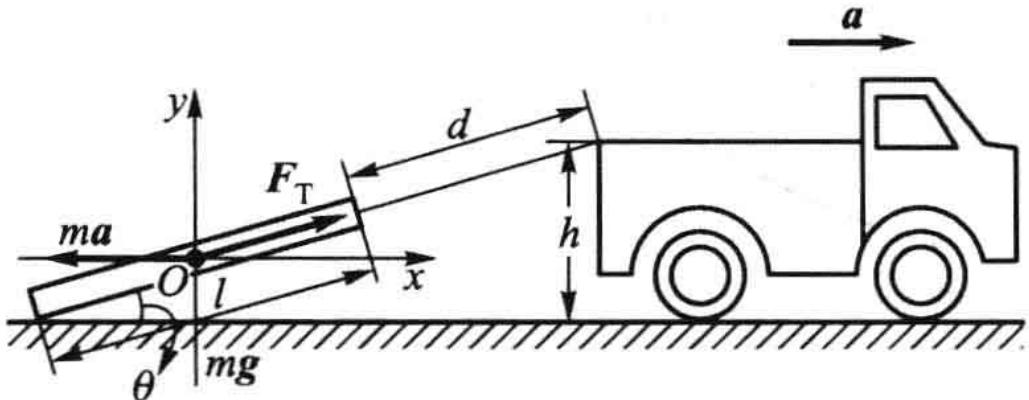
\includegraphics[width=0.4\textwidth]{figures/fig3-2.jpg}
  \end{figure}

\vfill
\newpage

\textbf{3-3.}在一体积为 $V$ , 质量为 $m_{0}$ 的铁盒内置有一阿特伍德机, 已知两物体的质量分别为 $m_{1}$ 和 $m_{2}$ 。现将此铁盒放入密度为 $\rho$ 的液体中, 如习题 3-3 图所示,试求铁盒在下沉过程中的加速度。忽略液体对铁盒的阻力作用。

\begin{figure}[H]
  \centering
  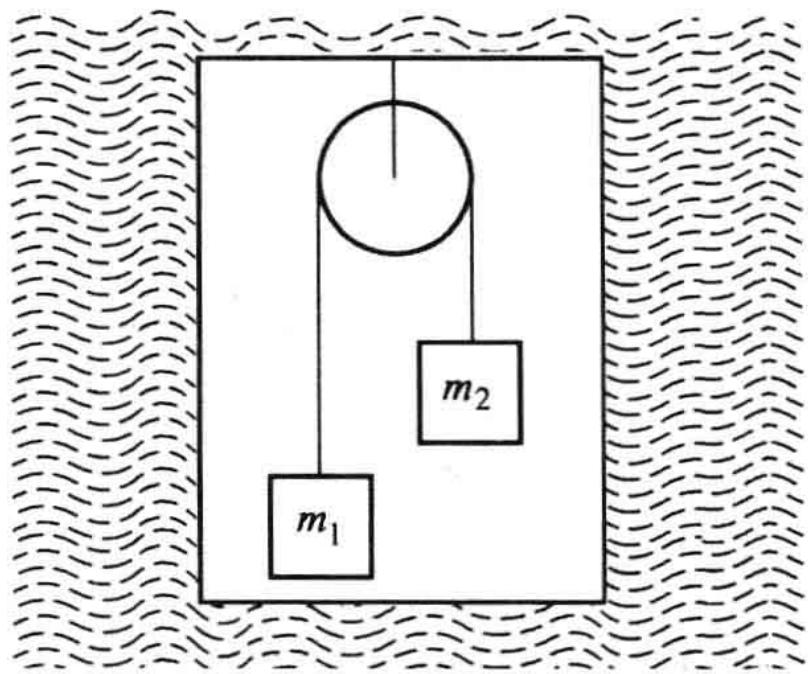
\includegraphics[width=0.25\textwidth]{figures/fig3-3.jpg}
  \end{figure}

\vfill

\textbf{3-4.}如习题 3-4 图所示, 质量为 $m_{2} = 2 \mathrm{~kg}$ 和 $m_{3} = 1 \mathrm{~kg}$ 的两个物体分别系在一根跨过滑轮 B 的细绳的两端, 而滑轮 B 又与质量为 $m_{1} = 3 \mathrm{~kg}$ 的物体系在另一根跨过定滑轮 A 的细绳的两端。试求:

(1) $m_{1}, m_{2}$ 和 $m_{3}$ 的加速度 $a_{1}, a_{2}$ 和 $a_{3}$ ;

(2) 跨过滑轮 A 的绳和跨过滑轮 B 的绳中张力 $F_{TA}$ 、 $F_{TB}$ 。

\vfill
\newpage

\textbf{3-5.}一质量为 $m_{0}$ , 倾角为 $\theta$ 的斜面体放在水平面上, 在斜面体上有一质量为 $m$ 的物体。为使 $m$ 不与斜面发生相对运动, 现用一水平力 $F$ 作用在 $m_{0}$ 上, 如习题 3-5 图所示。

(1) 若所有接触面均光滑, $F$ 应为多大?

(2) 若 $m$ 与 $m_0$ 之间的摩擦因数为 $\mu$ , 而 $m_0$ 与水平面间无摩擦, 求 $F$ 的范围。

\begin{figure}[H]
  \centering
  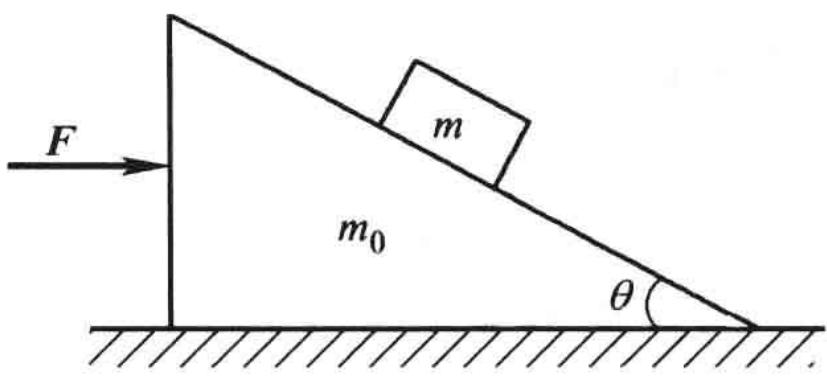
\includegraphics[width=0.4\textwidth]{figures/fig3-5.jpg}
  \end{figure}

\vfill

\textbf{3-6.}一摩托车以 $36 \mathrm{~km} / \mathrm{h}$ 的速率在地面上行驶。其轮胎与地面间的摩擦因数 $\mu$ 为0.3。试求：

(1) 摩托车在转弯时轨道的最小曲率半径;

(2) 摩托车与竖直线之间的最大倾斜角。

\vfill
\newpage

\textbf{3-7.}一根绳子的两端分别固定在顶板和底板上,两固定点位于同一竖直

线,相距为 $h$ 。一质量为 $m$ 的小球系于绳上某点处,当小球两边的绳均被拉直时,两绳与竖直线的夹角分别为 $\theta_{1}$ 和 $\theta_{2}$ ,如习题3-7图所示。当小球以一定的速度在水平面内做匀速圆周运动时,两绳均被拉直。试问:

(1) 若下面的绳子中的张力为零, 则小球的速度为多大?

(2) 若小球的速度是(1)小题中求得的速度的 $\sqrt{2}$ 倍, 则上、下两段绳中的张力各为多大?

\begin{figure}[H]
  \centering
  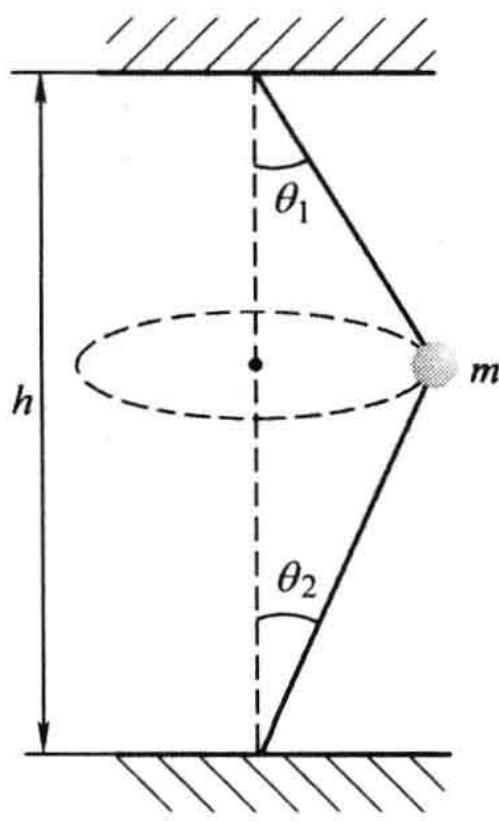
\includegraphics[width=0.2\textwidth]{figures/fig3-7.jpg}
  \end{figure}

\vfill

\textbf{3-8.}一小物体放在一半径为 $R$ 的水平圆盘边缘上, 小物体与圆盘间的静摩擦因数为 $\mu$ 。若圆盘绕其轴的角速度逐渐增大到一个值时, 小物体滑出圆盘并最终落到比盘面低 $h$ 的地面上。问从它离开圆盘的那一点算起, 小物体越过的水平距离多大?

\vfill
\newpage

\textbf{3-9.}一根光滑的钢丝弯成如习题3-9图所示的形状, 其上套有一小环。当钢丝以恒定角速度 $\omega$ 绕其竖直对称轴旋转时, 小环在其上任何位置都能相对静止。求钢丝的形状 (即写出 $y$ 与 $x$ 的关系)。

\begin{figure}[H]
  \centering
  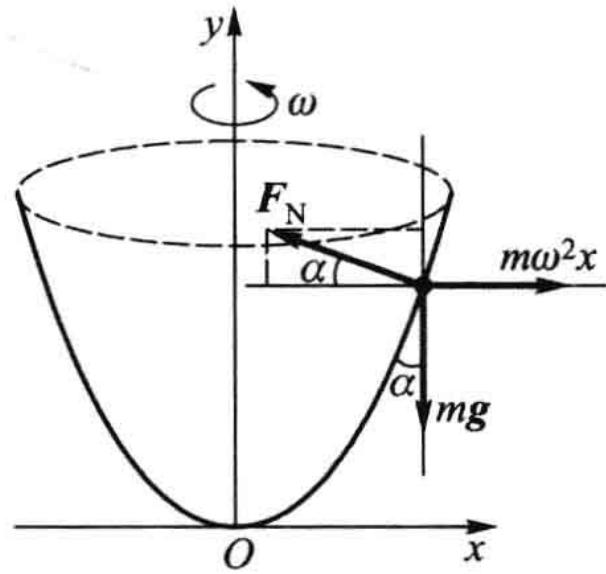
\includegraphics[width=0.3\textwidth]{figures/fig3-9.jpg}
  \end{figure}

\vfill

\textbf{3-10.}一圆盘绕其竖直的对称轴以恒定的角速度 $\omega$ 旋转。在圆盘上沿径向开有一光滑小槽, 槽内一质量为 $m$ 的质点以 $v_{0}$ 的初速从圆心开始沿半径向外运动。试求:

(1) 质点到达习题 3-10 图所示位置 (即 $y = y_0$ ) 时相对圆盘的速度 $v$ ;

(2) 质点到达该处所需要的时间 t;

(3) 质点在该处所受到的槽壁对它的侧向作用力 $F$ 。

\begin{figure}[H]
  \centering
  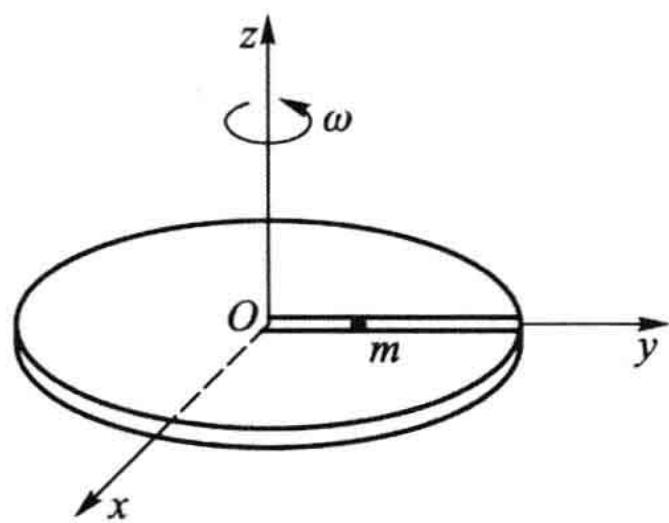
\includegraphics[width=0.3\textwidth]{figures/fig3-10.jpg}
  \end{figure}

\vfill
\newpage


\textbf{3-11.}在如习题 3-11 图所示的装置中, 质量分别为 $m_{2}$ 和 $m_{3}$ 的两物体由一细绳相连。细绳跨过装在一质量为 $m_{1}$ 的大物体上的定滑轮。已知所有的表面都光滑。试问:

(1) $m_{1}$ 的加速度为多大?

(2) 若在 $m_{1}$ 上作用一水平力 F，使 $m_{2}$ 和 $m_{3}$ 相对 $m_{1}$ 静止，则 F 为多大？

\begin{figure}[H]
  \centering
  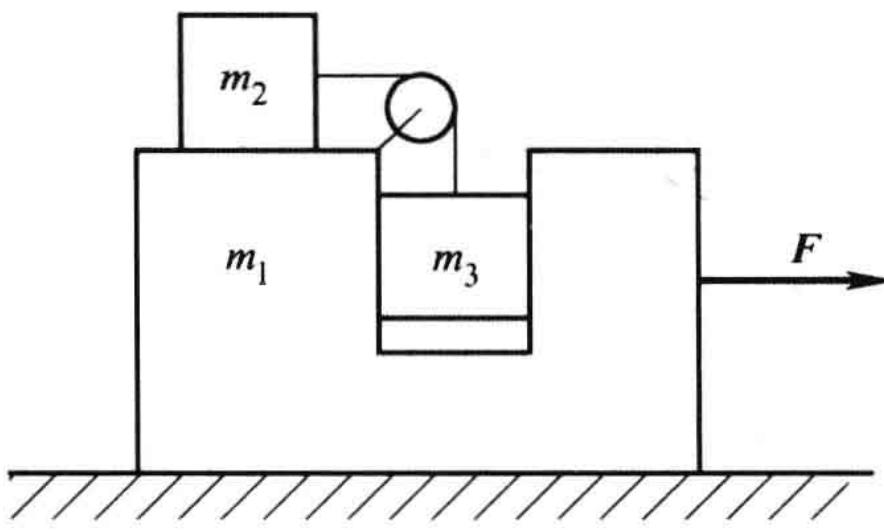
\includegraphics[width=0.3\textwidth]{figures/fig3-11_1.jpg}
  \end{figure}

\vfill

\textbf{3-12.}一个侧面边长比为 $3:4:5$ 的斜面固连在一转盘上, 如习题 3-12 图所示, 一木块静止在斜面上, 斜面和木块之间的摩擦因数 $\mu = \frac{1}{4}$ 。求此木块能保持在离转盘中心的水平距离为 $40 \mathrm{~cm}$ 处相对转盘不动的最小转动角速度 $\omega$ 。

\begin{figure}[H]
  \centering
  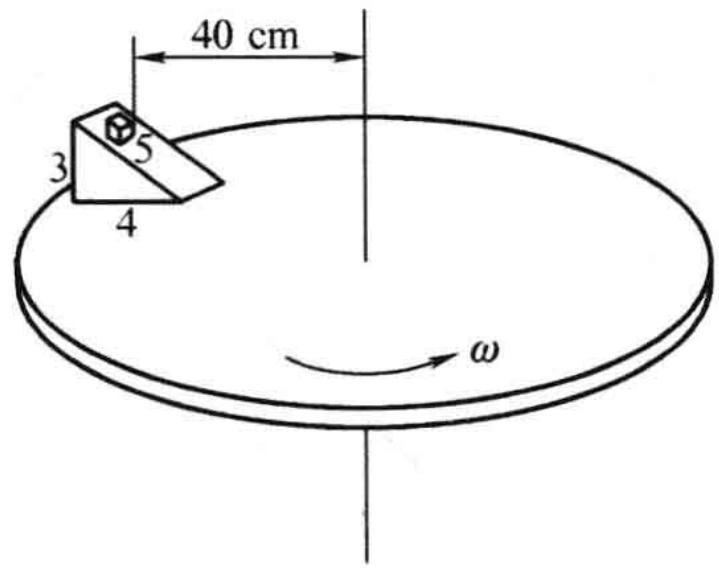
\includegraphics[width=0.25\textwidth]{figures/fig3-12.jpg}
  \end{figure}

\vfill
\newpage

\textbf{3-13.}一辆汽车驶入曲率半径为 $R$ 的弯道, 弯道倾斜一角度 $\theta$ , 车轮与路面之间的摩擦因数为 $\mu$ 。求汽车在路面上不侧向滑动时的最大和最小速度。

\vfill

\textbf{3-14.}一半顶角为 $\alpha$ 的竖直倒立圆锥面, 圆锥面以恒定的角速度 $\omega$ 绕其对称轴旋转。在圆锥内表面距轴为 $r$ 处有一质点。

（1）若圆锥面内表面光滑，要使质点随锥面一起匀速转动，即与锥面相对静止，求 $\omega$ 的值；

(2) 若质点与锥面间的摩擦因数为 $\mu$ , 为使质点相对锥面静止, 求 $\omega$ 的范围。

\vfill
\newpage

\textbf{3-15.}质量分别为 $m$ 及 $m'$ 的两个质点, 用未伸缩时长度为 $a$ 的弹性绳相连, 绳的劲度系数 $k = \frac{2mm' \omega^2}{m + m'}$ 。将此系统放在光滑的水平管内, 管子绕通过管上某点的竖直轴以恒定角速度 $\omega$ 转动。开始时, 两质点相对于管子是静止的, 两质点间距为 $a$ 。试求此后任何时刻两质点间的距离。

\vfill

\textbf{3-16.}质量为 $m$ 的小环套在半径为 $a$ 的光滑圆圈上, 可在其上滑动。如圆圈在水平面内以恒定角速度 $\omega$ 绕圈上某点 $O$ 转动, 转轴垂直于水平面, 如习题 3-16 图所示, 试求小环沿圆圈切线方向的运动微分方程。

\begin{figure}[H]
  \centering
  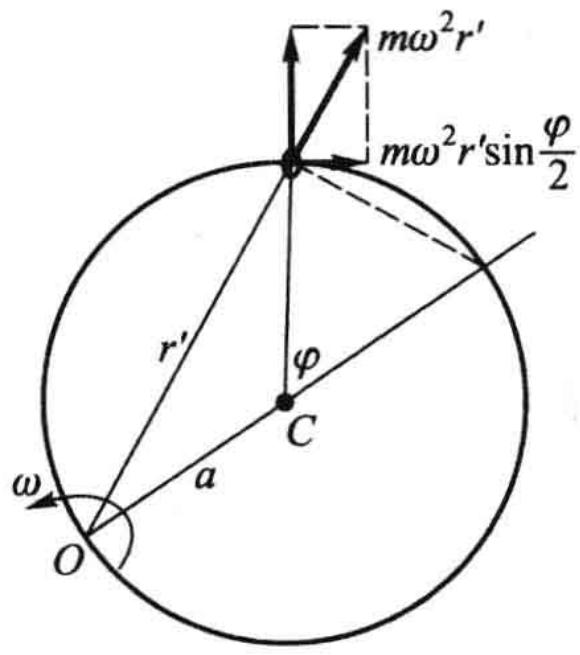
\includegraphics[width=0.25\textwidth]{figures/fig3-16.jpg}
  \end{figure}

\vfill
\newpage

\textbf{3-17.}质量为 $m$ 的小球置于光滑水平台面, 用长为 $l$ 的细绳系于台面上的 $P$ 点, 水平台面绕着过 $O$ 点的竖直轴以恒定角速度 $\omega$ 旋转, $P$ 点与 $O$ 点的距离为 $d$ 。试列出小球的运动方程。设在小球运动过程中, 绳始终保持拉直状态。

\begin{figure}[H]
  \centering
  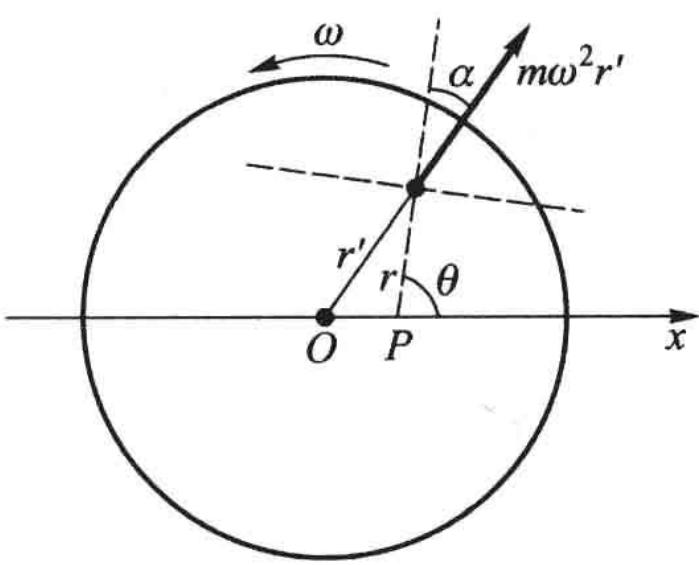
\includegraphics[width=0.3\textwidth]{figures/fig3-17.jpg}
  \end{figure}

\vfill

\textbf{3-18.}一圆柱形刚性杆 $OA$ 上套有一质量为 $m$ 的小环, 杆的一端固定, 整个杆绕着通过固定端 $O$ 的竖直轴以恒定的角速度旋转, 旋转时杆与竖直方向的夹角 $\alpha$ 保持不变。设小环与杆之间的摩擦因数为 $\mu$ , 已知当小环相对杆运动到习题 3-18 图所示的位置 $x$ 时, 其相对于杆的速度为 $\dot{x}$ , 试列出此时小环沿杆的运动方程。(不要求解出此方程)
\vfill
\newpage